\documentclass{article}
\usepackage[utf8]{inputenc}
\usepackage{graphicx}
\usepackage{float}
\usepackage{xcolor}

\title{Series de Tiempo}
\author{Carlos Oswaldo Ochoa Bojorquez\\
Actividad 1\\
Departamento de Física\\
Universidad de Sonora}
\date{13 de enero de 2021}

\begin{document}

\maketitle

\section{Introdución}
Para esta actividad recopilamos la información obtenida de una estación meteorológica la cual fue seleccionada por el estudiante, hubo un rango amplio para seleccionar la estación, por lo que yo escogí una ubicada en el lugar donde nací, Magdalena de Kino, Sonora, además de que cumple con las condiciones establecidas por el profesor, toda la información obtenida fue por medio de datos proporcionados por la  Comisión Nacional del Agua (CONAGUA).

\section{Datos de la estación}
\begin{center}
\begin{tabular}{|c|c|} \hline
   \textbf{Estación}  & \textcolor{red}{26160} \\ \hline
    \textbf{Nombre} & El Vivero \\ \hline
    \textbf{Estado} & Sonora \\ \hline
    \textbf{Municipio}& Magdalena de Kino \\ \hline
    \textbf{Latitud} & 30.6269° \\ \hline
    \textbf{Longitud} & \textcolor{red}{-110.9675°} \\ \hline
    \textbf{Altura} & 750 msnm \\ \hline
    \textbf{Situación} & Operando \\ \hline
    \textbf{Datos desde} & 1 de enero de 1969 \\ \hline
    \textbf{Hasta} & 30 de abril de 2016 \\ \hline
\end{tabular}    
\end{center}

\section{Datos de la ciudad}
Magdalena de Kino es un pueblo ubicado al norte de sonora, a 80 km de la frontera, este pueblo fue fundado por el misionero jesuita de origen italiano Eusebio Francisco Kino al rededor de 1687, todo esto con el fin de evangelizar a los nativos de estas tierras, es considerado uno de los pueblos mágicos de México por su relevancia histórica y cultural. El Pueblo Mágico de Magdalena se comunica, al oeste, con la ciudad de Caborca siguiendo por la carretera federal núm. 2; al norte con Nogales y Cananea, tomando la carretera federal núm. 15.

\begin{figure}[H]
    \centering
    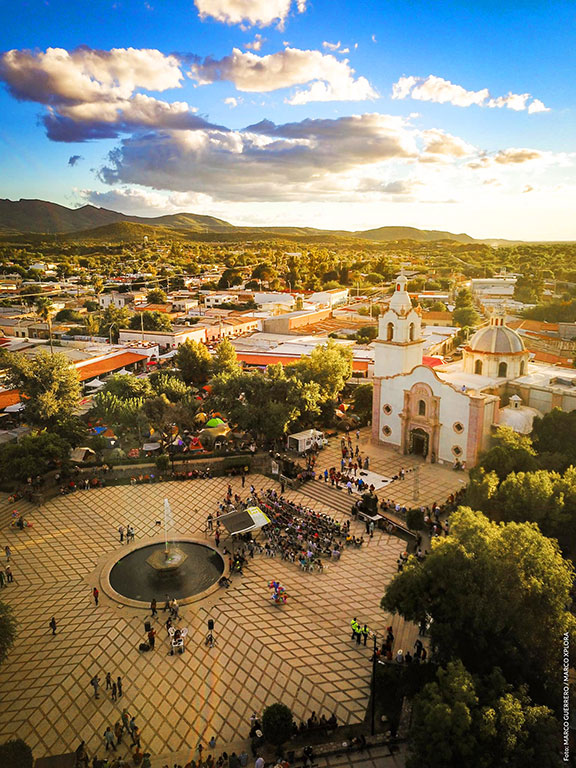
\includegraphics[height=15cm]{Fotos/Magdalena de kino.jpg}
    \caption{Imágen de la plaza de Magdalena.}
\end{figure}

\begin{figure}[H]
    \centering
    \includegraphics[height=10cm]{Fotos/Magdalena de Kino ubicación.png}
    \caption{Ubicacíon de Magdalena de Kino.}
\end{figure}

\section{Gráficas obtenidas en el reporte de estadística y observaciones hechas de estas mismas}

\begin{figure}[H]
    \centering
    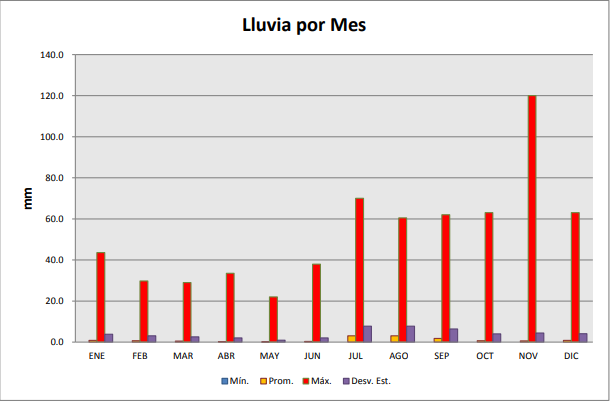
\includegraphics[height=8cm]{Fotos/Lluvia por mes.PNG}
    \caption{Lluvia por mes. \\
    \\
    Como se puede ver en esta gráfica, la lluvia promedio en Magdalena tiende a ser muy baja, ya que se trata de una zona desértica, pero esto no implica que en ciertas epocas del año llueva bastante.}
\end{figure}

\begin{figure}[H]
    \centering
    \includegraphics[height=8cm]{Fotos/Evaporación por mes.PNG}
    \caption{Evaporación por mes. \\
    \\
    Debido a las grandes temperaturas que se viven en el verano y primavera, la evaporación por mes aumenta en gran medida entre los meses de abril y julio, ya que en esos meses es cuando se registran temperaturas más altas, en cambio en el invierno esta evaporación baja considerablemente.}
\end{figure}

\begin{figure}[H]
    \centering
    \includegraphics[height=8cm]{Fotos/Promedio y máxino de lluvia.PNG}
    \caption{Promedio y máximo de precipitación.\\
    \\
    En esta gráfica podemos apreciar que a finales de los años 90 se vio una gran lluvia rompiendo record en el municipio de Magdalena, se alcanzaron los 120 mm, tanto en los años anteriores como posteriores, la lluvia se mantuvo a nivel medio.}
\end{figure}

\begin{figure}[H]
    \centering
    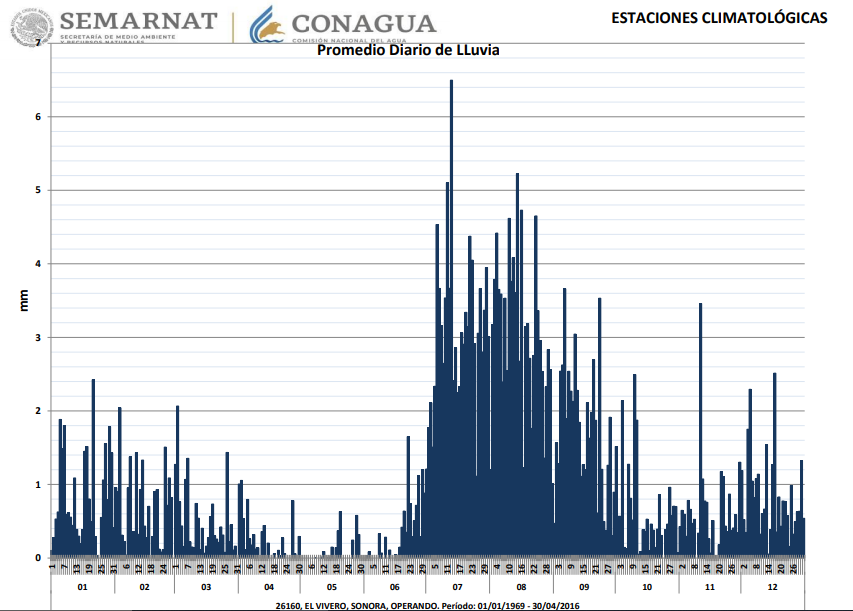
\includegraphics[height=8cm]{Fotos/Promedio diario de lluvia.PNG}
    \caption{Promedio de lluvias diarias.\\
    \\
    Entre los meses de julio y agosto es donde llueve más por día, se puede apreciar que, aunque en junio llueve más, estas lluvias tienden a ser muy fuertes y pocas, en contraste a este mes, en julio llueve muchos días pero no son lluvias fuertes como en junio.}
\end{figure}

\begin{figure}[H]
    \centering
    \includegraphics[height=8cm]{Fotos/Distribución de lluvia.PNG}
    \caption{Distribución de lluvia en rangos de 5 mm.\\
    \\
    Aquí podemos apreciar el rango de precipitación, el cual, si bien no es alto, tampoco es bajo.}
\end{figure}

\begin{figure}[H]
    \centering
    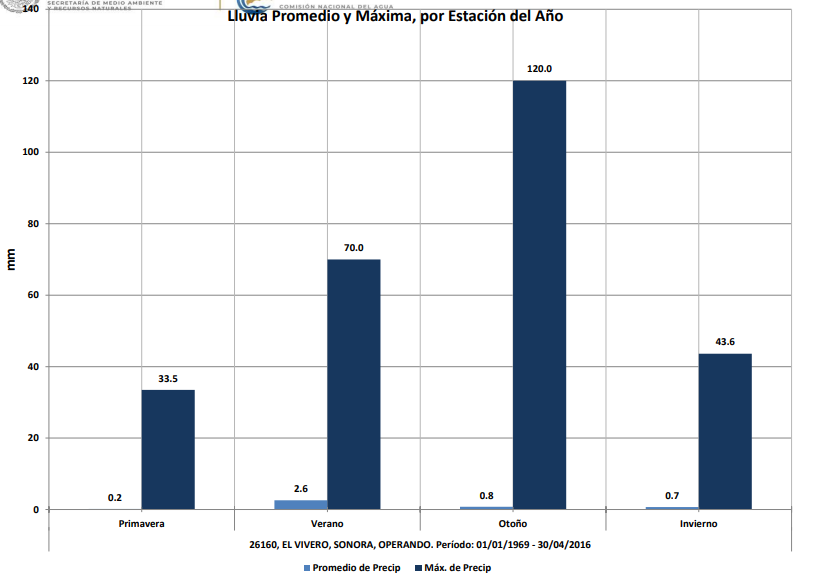
\includegraphics[height=8cm]{Fotos/Lluvia por estación del año.PNG}
    \caption{LLuvia promedio y máxima por estación del año.\\
    \\
    Se puede apreciar que en el verano se presenta un promedio mayor de lluvia mientras que en otoño hay un valor mayor de lluvia máxima.}
\end{figure}

\begin{figure}[H]
    \centering
    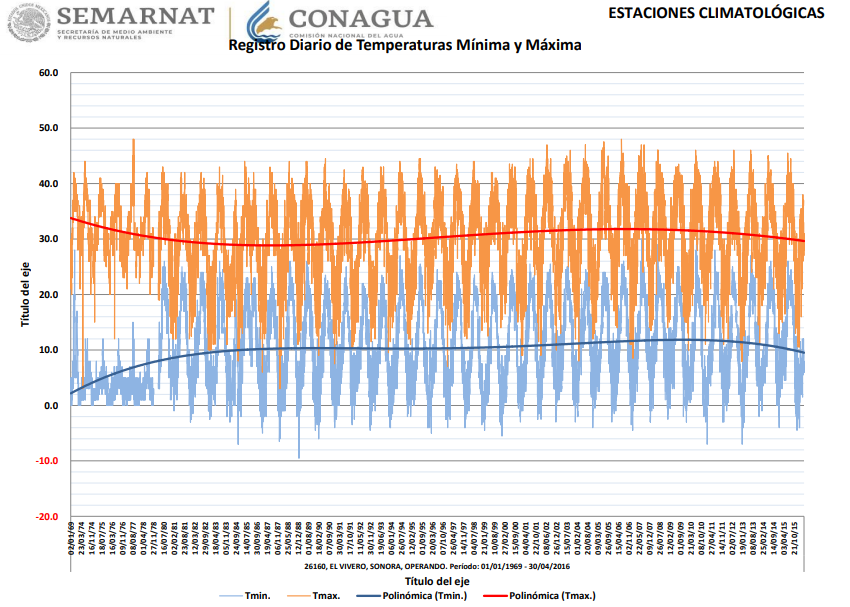
\includegraphics[height=8cm]{Fotos/Registro diario de temperatura máxima y mínima.PNG}
    \caption{Registro diario de temperaturas Máxima y Mínima.\\
    \\
    En la siguiente tabla podemos ver las variaciones que ocurren en la temperatura, estas llegan a ser tanto muy altas y muy bajas, debido a la zona desértica donde se encuentra el municipio, esto es algo común en ese tipo de zonas climáticas.}
\end{figure}

\begin{figure}[H]
    \centering
    \includegraphics[height=8cm]{Fotos/Temperatura máxima promedio mensual.PNG}
    \caption{Temperatura Máxima promedio mensual.\\
    \\
    Como podemos ver en esta gráfica, la temperatura máxima no llega a ser tan alta como Hermosillo, pero la temperatura mínima si llega a ser un tanto baja.}
\end{figure}

\begin{figure}[H]
    \centering
    \includegraphics[height=8cm]{Fotos/Temperatura mínima promedio mensual.PNG}
    \caption{Temperatura Mínima promedio mensual\\
    \\
    En cambio, en esta gráfica notamos que la temperatura mínima no llega a ser tan baja pero el promedio si lo es.}
\end{figure}

\begin{figure}[H]
    \centering
    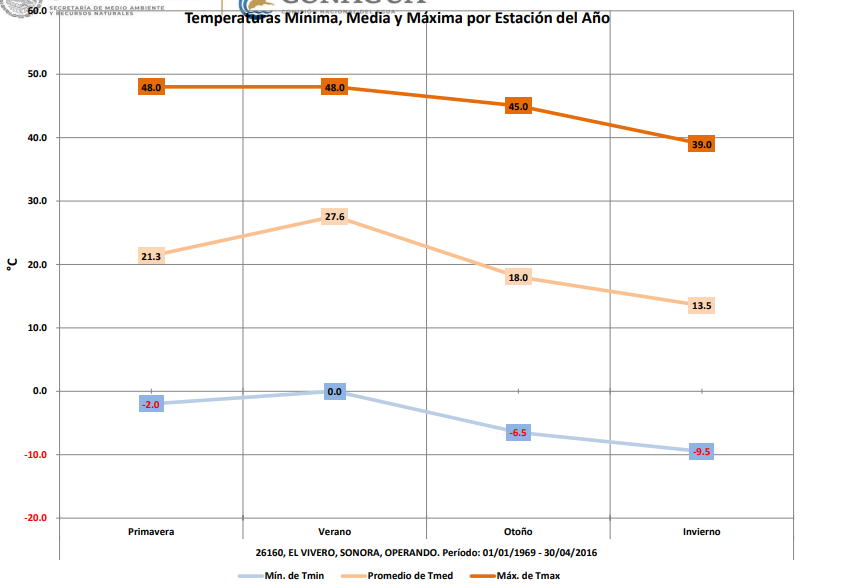
\includegraphics[height=8cm]{Fotos/Temperatura por estación del año.PNG}
    \caption{Temperatura mínima, media y máxima por estación del año.\\
    \\
    Como era de esperarse, en la primavera y verano se alcanzan temperaturas muy altas mientras que en el otoño e invierno temperaturas muy bajas.}
\end{figure}

\begin{figure}[H]
    \centering
    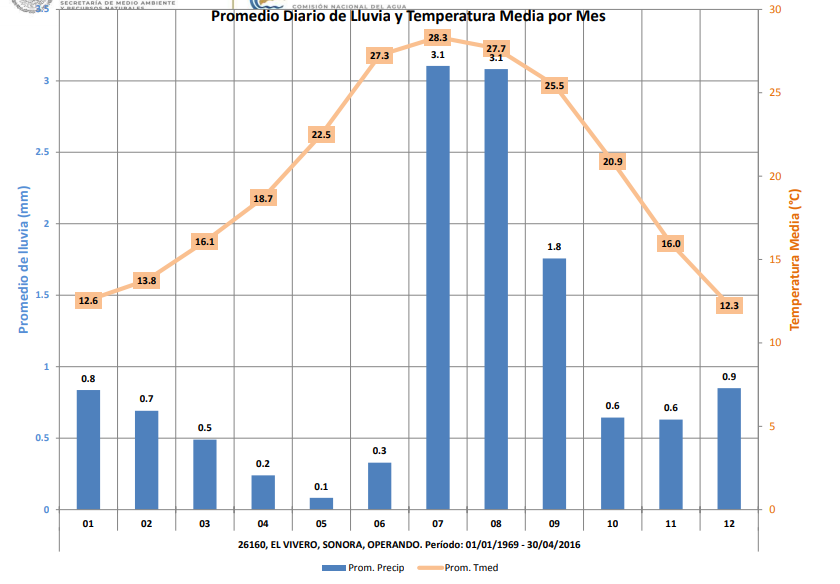
\includegraphics[height=8cm]{Fotos/Promedio diario de lluvia y temperatura media por mes.PNG}
    \caption{Promedio diario de lluvia y temperatura media por mes.\\
    \\
    Siendo un contraste bastante interesante, en el mes de julio es en el que se alcanza el mayor promedio de lluvia diaria y la temperatura media más alta.}
    
    \section{Primeras impresiones de la actividad desarrollada}
    
    Al inicio pensé que sería una actividad un tanto tediosa, ya que nunca antes habia utilizado LaTeX, pero esto no fue así, me di cuenta que este procesador de textos no es tan complicado como creía y su utilidad es muy grande. En cuanto al tema de la actividad me gustó mucho, pude conocer más acerca del clima de la ciudad donde nací, además de enterarme que habia estaciones meteorológicas en este municipio.
    
    \section{Opinión sobre la actividad}
    
    ¿Qué te pareció?
    \textcolor{blue}{Fue una actividad bastante interesante y resultó ser de mi agrado.}
    
    ¿Cómo estuvo el reto?
    \textcolor{blue}{Si bien al principio pensé que sería complicado, resultó ser lo contrario.}
    
    ¿Qué se te dificultó más?
    \textcolor{blue}{La parte que más se me dificultó fue la de acomodar las fotos en el pdf.}
    
    ¿Qué te aburrió?
    \textcolor{blue}{Toda la actividad fue bastante interesante, pero lo que me aburrió fue cuando tuve que seleccionar todas las gráficas de los datos de la estación.}
    
    ¿Qué recomendarías para mejorar esta actividad?
    \textcolor{blue}{Para mi fue una actividad bastante entretenida, no logro pensar algo que pueda mejorarla, tal vez subir un poco la dificultad.}
    
    ¿Qué grado de complejidad le asignarías a esta actividad? (Bajo, Intermedio, Avanzado)
    \textcolor{blue}{Bajo}
    
\end{figure}

\end{document}
